\titre{Exercice 1 :}
\begin{enumerate}
	\item Condition de concurrence : le résultat final dépend de l'ordonnancement
	\item Section critique : portion de code où deux processus ne devraient jamais se trouver en même temps sous peine de créer une condition de concurrence.
\end{enumerate}

\titre{Exercice 2}
\begin{enumerate}
	\item La création d'un thread est plus rapide que la création d'un processus.
	\item Pour être le plus général possible. Pour plusieurs variables on crée une struct. (idée : créer une fonction bidon qui va répartir les champs de la struct en argument et appeler la fonction qu'on veut)
	\item Il sert à enregistrer le retour d'une fonction.
	\item La valeur renvoyée par pthread\_join et pthread\_create est 0 pour un succès, autre chose pour une erreur.
\end{enumerate}

\titre{Exercice 3}
\begin{enumerate}
	\item 1,5 secondes
	\item 15 + 100*75 = 7515
	\item 100*15 + 10*75 = 2250 \\ 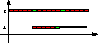
\includegraphics[width=200px]{fig8.pdf}
	\item 1,5 secondes \\ 
\includegraphics[width=200px]{fig9.pdf}
\end{enumerate}

\titre{Exercice 4}
\begin{enumerate}
	\item Un thread peut s'activer sur les requetes en cache pendant qu'un autre attend le disque dur
	\item L'appel à pthread\_create échouera si on dépasse le nombre maximal de thread autorisé
	\item  .\\ 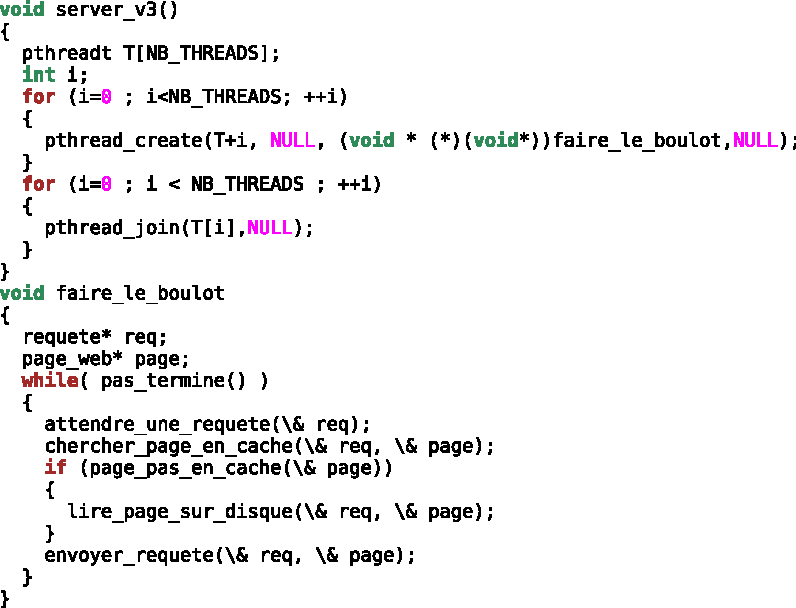
\includegraphics[width=300px]{fig10.pdf}

\end{enumerate}

\titre{Exercice 5 :} 
\begin{enumerate}
	\item $A1, A2, A3, A4, A5, B1, B2, B3, B4, B5, B6, B7, A6, A7$
	\item La section critique est composée des lignes 4 à 6
	\item Inverser les lignes 5 et 6 (la copie du document n'a pas besoin d'être en section critique.
\end{enumerate}

\titre{Exercice 6 :} \\

\includegraphics[width=300px]{fig11.pdf}
